\section{Versuchsbeschreibung}

In diesem Versuch geht es darum drei Materialien mit einem Rastertunnelmikroskop zu untersuchen, nämlich Gold, Graphit und Molybdändisulfid. Die Spitze wird selber aus einem PtIr-Draht angefertigt und mit einer Kneifzange gespitzt, so dass sie idealerweise einen atomaren Durchmesser hat. Diese wird dann in das Rastertunnelmikroskop eingesetzt und damit sollen die vorgefertigten Proben gemessen werden. Für  jede Probe sollen jeweils unterschiedliche Auflösungen gemessen und interpretiert werden.

\subsection{Der Aufbau}

\begin{figure}[H]
	\centering 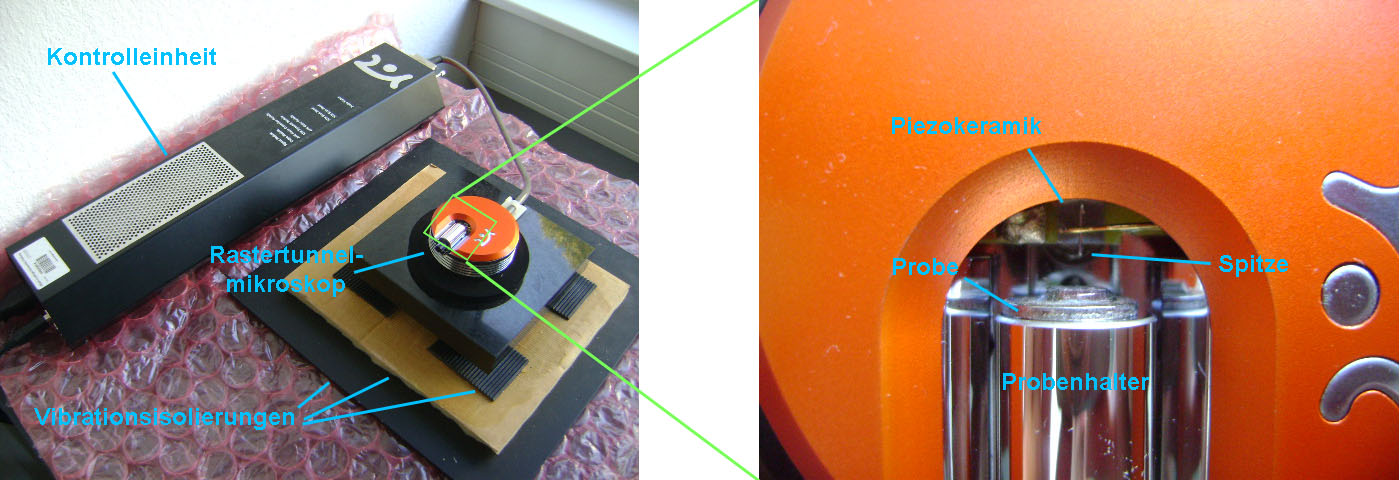
\includegraphics[width=\textwidth]{Bilder/aufbau.jpg}
	\caption{Versuchsaufbau}
\end{figure}

Die Gesamtheit des Rastertunnelmikroskops besteht aus dem Mikroskop selber, dessen Vibrationsisolierung, einer Kontrolleinheit, sowie der Probe, dem Probenhalter, der Spitze und dem Mechanismus zum bewegen einer Spitze, hier ein Piezokristall (siehe Bild). Außerdem gehört zu dem Aufbau noch ein PC, mit dem die Daten eingelesen und verarbeitet werden können. 
An der Kontrolleinheit gibt es eine Leuchte, deren Funktion es ist, anzugeben wie nahe die Spitze an der Probe ist. Leuchtet diese orange, so ist die Spitze zu weit weg von der Probe. Falls sie rot leuchtet, ist die Spitze zu nahe, bzw. berührt die Probe. Falls die Lampe grün leuchtet, so ist die Spitze genau so weit weg, dass der eingestellte Tunnelstrom erreicht wurde. Die Farbe dieser Leuchte haben wir bei jedem Annäherungsversuch der Spitze an die Probe dokumentiert und ist so bei jedem einzelnen Schritt in der Durchführung einzusehen.

\clearpage